\subsection{BÀI TẬP TRẮC NGHIỆM}
\Opensolutionfile{ans}[ans/ansTL-0D2-B2]
\setcounter{ex}{0}
\begin{ex}%[Ninh Tiến Nam - Dự án 2019-THPTMaT-1]%[0D4K4-2]%
	Cho hệ bất phương trình $\begin{cases}
		x+2y-3<0\\
		2x+y-2>0
	\end{cases}$. Điểm nào sau đây thuộc miền nghiệm của hệ bất phương trình đã cho?
	\choice
	{$Q(-1;-5)$}
	{$N(2;2) $}
	{\True$P(3;-1) $}
	{$M(2;3)$}
	\loigiai{
		Thay tọa độ từng điểm vào ta thấy chỉ có điểm $P(3;-1)$ thỏa hai bất phương trình của hệ.}
\end{ex}

\begin{ex}%[0D4B4]
	Cho hệ bất phương trình $\heva{&y\geq0\\&3x+2y-6<0}$ có miền nghiệm là $S$ và bốn điểm $O(0;0)$, $A(2;3)$, $B(-1;1)$, $C(-1;3)$. Có bao nhiêu điểm thuộc $S$?
	\choice{1}
	{2}
	{\True 3}
	{4}
	\loigiai{
		Thay tọa độ các điểm đã cho vào hệ, ta được các điểm $O$, $B$, $C$ thỏa.
	}
\end{ex}

\begin{ex}%[0D4Y4-4]
	Miền nghiệm của hệ bất phương trình $\heva{&2x-5y-1>0\\&2x+y+5>0\\&x+y+1<0}$ chứa điểm nào trong các điểm sau?
	\choice
	{$(0;0)$}
	{$(1;0)$}
	{\True $(0;-2)$}
	{$(0;2)$}
	\loigiai{Thay điểm $(0;-2)$ vào hệ bất phương trình, ta có 
		$\heva{&2 \cdot 0 - 5 \cdot (-2)-1=9>0\\&2 \cdot 0 + (-2) +5=3>0\\&0+(-2)+1=-1<0}$ (đúng).
	}
\end{ex}

\begin{ex}%[0D4Y4-4]
	Miền nghiệm của hệ bất phương trình $\heva{& x-y\ge 3 \\ & 2x+y<4}$ chứa điểm nào trong các điểm sau?
	\choice
	{\True $(1;-3)$}
	{$(-2;1)$}
	{$(3;-2)$}
	{$(4;1)$}
	\loigiai{Thay điểm $(1;-3)$ vào hệ bất phương trình, ta có
		$\heva{& 1-(-3) = 4 \ge 3 \\ & 2 \cdot 1 + (-3) = -2 <4}$ (đúng).
	}
\end{ex}

\begin{ex}%[0D4B4-4]
	Miền nghiệm của hệ bất phương trình $\heva{& 2x-y>0\\ & x+y\ge -1 \\ & x-y<-2}$ \textbf{không} chứa điểm nào trong các điểm sau?
	\choice
	{$(5;8)$}
	{$(6;9)$}
	{$(4;7)$}
	{\True $(3,4)$}
	\loigiai{Thay điểm $(3;4)$ vào hệ bất phương trình, ta có
		$\heva{& 2 \cdot 3 - 4 = 2>0 \\ & 3+4=7 \ge -1 \\ & 3-4 = -1<-2}$ (sai).
	}
\end{ex}

\begin{ex}%[0D4K4-2]
	Tính diện tích $S$ của miền nghiệm hệ bất phương trình $\heva{& y+x\le 3 \\ & y-x\le 3 \\ & y\ge -1}$.
	\choice
	{$S=8$}
	{$S=25$}
	{\True $S=16$}
	{$S=12$}
	\loigiai{
		\immini{
			Miền nghiệm là miền tam giác như hình vẽ.\\
			Diện tích $S=\dfrac{1}{2}.8.4=16$
		}
		{
			\begin{tikzpicture}[scale=0.5, font=\footnotesize, line join=round, line cap=round, >=stealth]
				\def\xmin{-5} \def\xmax{5}
				\def\ymin{-2} \def\ymax{4}
				\clip(\xmin,\ymin) rectangle (\xmax,\ymax);
				\tkzDefPoints{\xmax/\ymax/A1,\xmin/\ymax/A2,\xmin/\ymin/A3,\xmax/\ymin/A4}
				\fill[pattern=north east lines,pattern color=black!60] (A1)--(A2)--(A3)--(A4)--cycle;
				\tkzDefPoints{-4/-1/M,0/3/I,4/-1/N}
				\fill[color=white] (M)--(I)--(N)--cycle;
				\draw[domain=-5:5] plot(\x,{3-(\x)}) plot(\x,{3+(\x)}) plot(\x,{-1});
				\begin{scriptsize}
					\draw[->](\xmin,0)--(\xmax,0); \draw(\xmax-0.1,0) node[below]{$x$};
					\draw[->](0,\ymin)--(0,\ymax); \draw(0,\ymax-0.2) node[right]{$y$};
					\foreach \x in {-4,4}
					\draw (\x,0.05) -- ++(0,-0.1) node [above] {$\x$};
					\draw node [above right]{$O$} (0,3) 
					node[left]{$3$} (0,-1) 
					node[below left]{$-1$};
					\draw[dashed] (-4,0)--(M) (4,0)--(N);
				\end{scriptsize}
			\end{tikzpicture}
		}
	}
\end{ex}

\begin{ex}%[0D4K4-2]
	Tính diện tích $S$ của miền nghiệm của hệ bất phương trình $\heva{& x\ge -3 \\ & y+x\le 8 \\ & y-x\ge -2}$.
	\choice
	{$S=48$}
	{\True $S=64$}
	{$S=81$}
	{$S=49$}
	\loigiai{
		\immini{
			Miền nghiệm là miền tam giác như hình vẽ.\\
			Diện tích $S=\dfrac{1}{2}.16.8=64$.
		}
		{
			\begin{tikzpicture}[scale=0.3, font=\footnotesize, line join=round, line cap=round, >=stealth]
				\def\xmin{-6} \def\xmax{9}
				\def\ymin{-6} \def\ymax{12}
				\clip(\xmin,\ymin) rectangle (\xmax,\ymax);
				\tkzDefPoints{\xmax/\ymax/A1,\xmin/\ymax/A2,\xmin/\ymin/A3,\xmax/\ymin/A4}
				\fill[pattern=north east lines,pattern color=black!60] (A1)--(A2)--(A3)--(A4)--cycle;
				\tkzDefPoints{-3/-5/M,-3/11/N,5/3/I}
				\fill[color=white] (M)--(N)--(I)--cycle;
				\draw[domain=-5:5] plot(\x,{8-(\x)}) plot(\x,{(\x)-2});
				\draw (-3,\ymin)--(-3,\ymax);
				\begin{scriptsize}
					\draw[->](\xmin,0)--(\xmax,0); \draw(\xmax-0.1,0) node[below]{$x$};
					\draw[->](0,\ymin)--(0,\ymax); \draw(0,\ymax-0.2) node[right]{$y$};
					\foreach \x in {-3,5}
					\draw (\x,0.05) -- ++(0,-0.1) node [above right] {$\x$};
					\foreach \x in {-5,3,11}
					\draw (0.05,\x) -- ++(-0.1,0) node [above left] {$\x$};
					\draw node [above right]{$O$};
					\draw[dashed] (M)--(0,-5) (N)--(0,11) (0,3)--(I)--(5,0);
				\end{scriptsize}
			\end{tikzpicture}
		}
	}
\end{ex}

\begin{ex}%[0D4K4-2]
	Tính chu vi $P$ của miền nghiệm hệ bất phương trình $\heva{& x\ge -3 \\ & x\le 6 \\& y\le 5 \\ & y\ge -6}$.
	\choice
	{$P=38$}
	{$P=36$}
	{$P=42$}
	{\True $P=40$}
	\loigiai{
		\immini{
			Miền nghiệm là miền hình chữ nhật như hình vẽ.\\
			Chu vi $P=2(11+9)=40$.
		}
		{
			\begin{tikzpicture}[scale=0.3, font=\footnotesize, line join=round, line cap=round, >=stealth]
				\def\xmin{-5} \def\xmax{8}
				\def\ymin{-8} \def\ymax{7}
				\clip(\xmin,\ymin) rectangle (\xmax,\ymax);
				\tkzDefPoints{\xmax/\ymax/A1,\xmin/\ymax/A2,\xmin/\ymin/A3,\xmax/\ymin/A4}
				\fill[pattern=north east lines,pattern color=black!60] (A1)--(A2)--(A3)--(A4)--cycle;
				\tkzDefPoints{-3/-6/M,-3/5/N,6/5/P,6/-6/Q}
				\fill[color=white] (M)--(N)--(P)--(Q)--cycle;
				\draw (-3,\ymin)--(-3,\ymax) (6,\ymin)--(6,\ymax) (\xmin,5)--(\xmax,5) (\xmin,-6)--(\xmax,-6);
				\begin{scriptsize}
					\draw[->](\xmin,0)--(\xmax,0); \draw(\xmax-0.1,0) node[below]{$x$};
					\draw[->](0,\ymin)--(0,\ymax); \draw(0,\ymax-0.2) node[right]{$y$};
					\foreach \x in {-3,6}
					\draw (\x,0.05) -- ++(0,-0.1) node [above right] {$\x$};
					\foreach \x in {-6,5}
					\draw (0.05,\x) -- ++(-0.1,0) node [above left] {$\x$};
					\draw node [above right]{$O$};
				\end{scriptsize}
			\end{tikzpicture}
		}	
	}
\end{ex}

\begin{ex}%[0D4K4-3]
	Ngoài giờ học, bạn Nam làm thêm việc phụ bán cơm được $15$ nghìn đồng/một giờ và phụ bán tạp hóa được $10$ nghìn đồng/một giờ. Nam không thể làm thêm việc nhiều hơn $15$ giờ mỗi tuần. Gọi $x$, $y$ lần lượt là số giờ phụ bán cơm và phụ bán tạp hóa. Hệ bất phương trình nào sau đây xác định số giờ để làm mỗi việc nếu Nam muốn kiếm được ít nhất $100$ nghìn đồng mỗi tuần?
	\def\dotEX{}
	\choice
	{$\heva{&x \ge 0\\& y \ge 0\\& x+y\ge 15\\& 15x+10y\ge 100.}$}
	{$\heva{&x \ge 0\\& y \ge 0\\& x+y\le 15\\& 15x+10y>100.}$}
	{\True $\heva{&x \ge 0\\& y \ge 0\\& x+y\le 15\\& 15x+10y\ge 100.}$}
	{$\heva{&x \ge 0\\& y \ge 0\\& x+y>15\\& 15x+10y<100.}$}
	\loigiai{
		Gọi $x$, $y$ lần lượt là số giờ phụ bán cơm và phụ bán tạp hóa, tổng số giờ này không được nhiều hơn $15$ giờ nên $x+y\le 15$.\\
		Số tiền kiếm được sau $x$ giờ phục vụ cơm là $15x$.\\
		Số tiền kiếm được sau $y$ giờ bán tạp hóa là $10y$.\\
		Để Nam kiếm được ít nhất 100 nghìn đồng mỗi tuần thì $15x+10y\ge 100.$\\
		Vậy ta có hệ $\heva{& x+y\le 15\\& 15x+10y\ge 100.}$
	}
\end{ex}

\begin{ex}%[0D4T4]
	Để trở thành một thành viên của ban nhạc thì một sinh viên phải đạt điểm trung bình các môn học ít nhất là $7,0$ và phải có tối thiểu $5$ lần thực hành sau giờ học. Hãy chọn hệ bất phương trình thể hiện tốt nhất tình huống này.
	\choice
	{\True $\heva{& x\ge 7 \\ & y\ge 5}$}
	{$\heva{& x\le 7 \\ & y\le 5}$}
	{$\heva{& x<7 \\ & y<5}$}
	{$\heva{& x>7 \\ & y>5}$}
	\loigiai{
	}
\end{ex}

\begin{ex}%[0D4K4-3]
	Để trở thành một thành viên của ban nhạc thì một sinh viên phải đạt điểm trung bình các môn học ít nhất là $7{,}0$ và phải có tối thiểu $5$ lần thực hành sau giờ học. Gọi $x$ là điểm trung bình các môn học và $y$ là số lần thực hành sau giờ học, hãy chọn hệ bất phương trình thể hiện tốt nhất tình huống này.
	\def\dotEX{}
	\choice
	{\True $\heva{& x\ge 7 \\ & y\ge 5.}$}
	{$\heva{& x\le 7 \\ & y\le 5.}$}
	{$\heva{& x<7 \\ & y<5.}$}
	{$\heva{& x>7 \\ & y>5.}$}
	\loigiai{
		Theo đề điểm trung bình các môn học ít nhất là $7,0$, tức là $x\ge 7$.\\
		Học sinh phải có tối thiểu $5$ lần thực hành sau giờ học, tức là $y\ge 5.$	\\
		Vậy ta có hệ $\heva{& x\ge 7 \\ & y\ge 5.}$
	}
\end{ex}

\begin{ex}%[0D4K4-4]
	\immini[thm]{Hình vẽ dưới đây là biểu diễn hình học tập nghiệm của hệ bất phương trình nào? (với miền nghiệm là miền \textbf{không} gạch sọc và chứa bờ)
	\choice
	{\True $\heva{&3x+4y-8 \geq 0 \\ &5x-12y-3\leq 0.}$}
	{$\heva{&3x+4y-8 \leq 0 \\ &5x-12y-3\leq 0.}$}
	{$\heva{&3x+4y-8 \geq 0 \\ &5x-12y-3 \geq 0.}$}
	{$\heva{&3x+4y-3 \geq 0 \\ &5x-12y-8 \leq 0.}$}}{
	\begin{tikzpicture}[line join=round, line cap=round, >=stealth,font=\footnotesize, scale=0.6]
		\draw[->](-3,0)--(4,0) node[below right] {$x$};
		\draw[->](0,-2)--(0,4) node[above] {$y$};
		\node (0,0) [above left]{$ O $};
		\foreach \x in {-2,...,2}
		\draw[shift={(\x,0)},color=black] (0pt,2pt) -- (0pt,-2pt);
		\foreach \y in {-1,...,3}
		\draw[shift={(0,\y)},color=black] (2pt,0pt) -- (-2pt,0pt);
		\draw[samples=100,smooth,domain=-2:4] plot(\x,{-0.75*(\x)+2});
		\draw[samples=100,smooth,domain=-3:4] plot(\x,{5/12*(\x)-1/4});
		\draw[dashed] (3,0)node[below] {$3$}--(3,1)--(0,1)node[left] {$1$};
		\fill[pattern=north east lines,pattern color=orange] (-2,3.5)--(-3,3.5)--(-3,-2)--(4,-2)--(4,-1);
		\fill[pattern=dots,pattern color=blue] (-3,-1.5)--(-3,-2)--(4,-2)--(4,1.416666);
		\node[right] at (0,2.1) {$2$};
\end{tikzpicture}}
	\loigiai{Xét các điểm $A(0; 2)$, $B (3; 1)$ và $C \left(0; - \dfrac{1}{4}\right)$ thuộc bờ. \\
		Điểm $B (3; 1)$ không thỏa mãn bất phương trình $3x+4y-8 \leq 0$ nên loại $\heva{&3x+4y-8 \leq 0 \\ &5x-12y-3\leq 0.}$ \\ 
		Điểm $A (0; 2)$ không thỏa mãn bất phương trình $5x - 12 y - 3 \geq 0$ nên loại $\heva{&3x+4y-8 \geq 0 \\ &5x-12y-3 \geq 0.}$\\
		Điểm $C \left(0; - \dfrac{1}{4}\right)$ không thỏa mãn bất phương trình $3x + 4y - 3 \geq 0$ nên loại $\heva{&3x+4y-3 \geq 0 \\ &5x-12y-8 \leq 0.}$
	}
\end{ex}

\begin{ex}%[0D4K4-4]
	\immini[thm]{Phần mặt phẳng không bị gạch, kể cả phần biên của nó trên đường thẳng $y=0$ trong hình vẽ bên là miền nghiệm của hệ bất phương trình nào?
		\def\dotEX{}
		\choice
		{$ \heva{&y\leq0\\ &2x+y>1.}$}
		{\True $ \heva{&x+y<2\\&y\geq0.}$}
		{$\heva{&2x-2y>6\\&2x+y\geq1.}$}
		{$ \heva{&y\leq0\\&x+y<1.}$}
	}{\begin{tikzpicture}[scale=0.7, font=\footnotesize, line join=round, line cap=round, >=stealth]
			\draw[->] (-1,0) -- (3.1,0)node[above]{$x$};
			\foreach \x in {1,2,3}
			\draw[shift={(\x,0)},color=black] (0pt,2pt) -- (0pt,-2pt) node[below] {\footnotesize $\x$};
			\draw[->,color=black] (0,-1) -- (0,3.1)node[right]{$y$};
			\foreach \y in {1,2,3}
			\draw[shift={(0,\y)},color=black] (2pt,0pt) -- (-2pt,0pt) node[left] {\footnotesize $\y$};
			\node[below left] at (0,0) {$O$};
			\fill[pattern=north east lines] (-1,3) -- (3,3) -- (3,-1) -- cycle;
			\draw[line width=1.2pt,smooth,samples=100,domain=-1:3] plot(\x,{2-(\x)});
			\fill[pattern=north east lines] (-1,0)--(-1,-1) --(3,-1)--(3,0)-- cycle;
		\end{tikzpicture}
	}
	\loigiai{Phần không bị gạch nằm phía trên trục hoành nên nó là miền nghiệm của bất phương trình $y \geq 0$ $(1)$. \\ 
		Điểm $A (0; 1)$ thỏa mãn bất phương trình $x + y < 2$ nên miền không bị gạch chính là miền nghiệm của bất phương trình $x +y < 2$ $(2)$. \\
		Từ $(1)$ và $(2)$ suy ra phần mặt phẳng không bị gạch, kể cả phần biên của nó trên đường thẳng $y=0$ trong hình vẽ bên là miền nghiệm của hệ bất phương trình $ \heva{&x+y<2\\&y\geq0.}$
	}
\end{ex}

\begin{ex}%[0D4K4-2]
	Xét $x$, $y$ thỏa mãn hệ bất phương trình $\heva{&x\ge 0 \\ & y\ge 0 \\& x+2y\le 4 \\& x-y\le 1.}$ Tìm giá trị lớn nhất $M$ của biểu thức $F=3x+2y$.
	\choice
	{\True $M=8$}
	{$M=10$}
	{$M=6$}
	{$M=9$}
	\loigiai{
		\immini{
			Miền nghiệm là tứ giác như hình vẽ.\\
			$F$ lớn nhất là $8$ tại đỉnh $(2;1)$.
		}
		{
			\begin{tikzpicture}[scale=0.7, font=\footnotesize, line join=round, line cap=round, >=stealth]
				\def\xmin{-1} \def\xmax{5}
				\def\ymin{-1.5} \def\ymax{3}
				\clip(\xmin,\ymin) rectangle (\xmax,\ymax);
				\tkzDefPoints{0/0/O,1/0/M,2/1/N,0/2/P}
				\tkzDrawPoints(O,M,N,P)
				\fill[pattern=north east lines,pattern color=blue!60] (O)--(M)--(N)--(P)--cycle;
				\draw[domain=-1:5] plot(\x,{2-(\x)/2}) plot(\x,{(\x)-1});
				\begin{scriptsize}
					\draw[->](\xmin,0)--(\xmax,0); \draw(\xmax-0.1,0) node[below]{$x$};
					\draw[->](0,\ymin)--(0,\ymax); \draw(0,\ymax-0.2) node[right]{$y$};
					\foreach \x in {1,2,4}
					\draw (\x,0.05) -- ++(0,-0.1) node [below] {$\x$};
					\foreach \x in {1,2}
					\draw (0.05,\x) -- ++(-0.1,0) node [left] {$\x$};
					\draw node [below left]{$O$};
				\end{scriptsize}
			\end{tikzpicture}
		}	
	}
\end{ex}

\begin{ex}%[0D4K4-2]%
	Xét $x$, $y$ thỏa mãn hệ điều kiện $\heva{&x-2y+2\geq0\\&3x+8y-24\leq0\\&x\geq0\\&y\geq0.}$ Tìm giá trị lớn nhất của biểu thức $F(x;y)=x-y-1$.
	\choice
	{$ 5 $}
	{\True$ 7 $}
	{$ 6 $}
	{$ 8 $}
	\loigiai{
		\immini{
			Dễ thấy rằng: miền nghiệm của hệ đã cho là hình tứ giác OABC trên hình vẽ (Kể cả biên), trong đó các đỉnh của tứ giác có tọa độ: $O (0;0)$, $A (0;1)$, $B \left(\dfrac{16}{7};\dfrac{15}{7} \right)$, $C (8;0)$.
		}
		{\begin{tikzpicture}[scale=1,thick,>=stealth']
				\draw[->] (-3,0) -- (8.3,0)node[above]{$x$};
				\foreach \x in {-3,-2,-1,1,2,3,4,5,6,7,8}
				\draw[shift={(\x,0)},color=black] (0pt,2pt) -- (0pt,-2pt) node[below] {\footnotesize $\x$};
				\draw[->,color=black] (0,-1) -- (0,4.3)node[right]{$y$};
				\foreach \y in {-1,1,2,3,4}
				\draw[shift={(0,\y)},color=black] (2pt,0pt) -- (-2pt,0pt) node[left] {\footnotesize $\y$};
				\clip(-3,-1) rectangle (8.3,4);
				\fill[pattern=north east lines] (-2,3.75) -- (-3,4) -- (8,4) -- (8,0)-- cycle;
				\draw[line width=1.2pt,smooth,samples=100,domain=-3:9] plot(\x,{3-0.375*(\x)});
				\fill[pattern=north east lines] (-3,4)--(-3,-0.5)--(6,4)--(8,4)-- cycle;
				\draw[line width=1.2pt,smooth,samples=100,domain=-3:9] plot(\x,{1+0.5*(\x)});
				\fill[pattern=north east lines] (0,4)--(-3,4) --(-3,-3)--(0,-3)-- cycle;
				%\draw[line width=1.2pt,smooth,samples=100,domain=-3:9] plot(\x,{0*(\x)});
				\fill[pattern=north east lines] (-3,0)--(-3,-3) --(8,-3)--(8,0)-- cycle;
				\color{red}{\node[below] at (2.285,2) {$B$};
					\node[below right] at (0,1) {$A$};
					\node[below left] at (8,0) {$C$};
					\node[above right] at (0,0) {$O$};
				}
			\end{tikzpicture}
		}
		\noindent Ta biết rằng giá trị lớn nhất của biểu thức $F(x;y)$ sẽ đạt được tại các đỉnh của tứ giác, do đó ta tính giá trị của $F(x;y)$ tại các đỉnh này.
		$F(0;0)=-1$, $F(0;1)=-2$, $F\left(\dfrac{16}{7};\dfrac{15}{7} \right)=-\dfrac{6}{7}$, $F(8;0)=7$. \\
		Vậy giá trị lớn nhất của biểu thức thỏa mãn hệ là $F(8;0)=7$.
	}
\end{ex}

\begin{ex}%[0D4G4-2]%
	Gọi $(x,y)$ là nghiệm của hệ bất phương trình $\heva{&x-2y-2\le 0\\&4x-3y+12\ge 0\\&x+3y+3\ge 0\\& 2x+y-4\le 0}$. Tìm giá trị lớn nhất của biểu thức $F=4x+5y-6$.
	\choice
	{$2$}
	{$18$}
	{$-18$}
	{\True $14$}
	\loigiai{
		Biểu diễn tập nghiệm của hệ bất phương trình $\heva{&x-2y-2\le 0\\&4x-3y+12\ge 0\\&x+3y+3\ge 0\\& 2x+y-4\le 0}$ trên mặt phẳng tọa độ ta được
		\begin{center}
			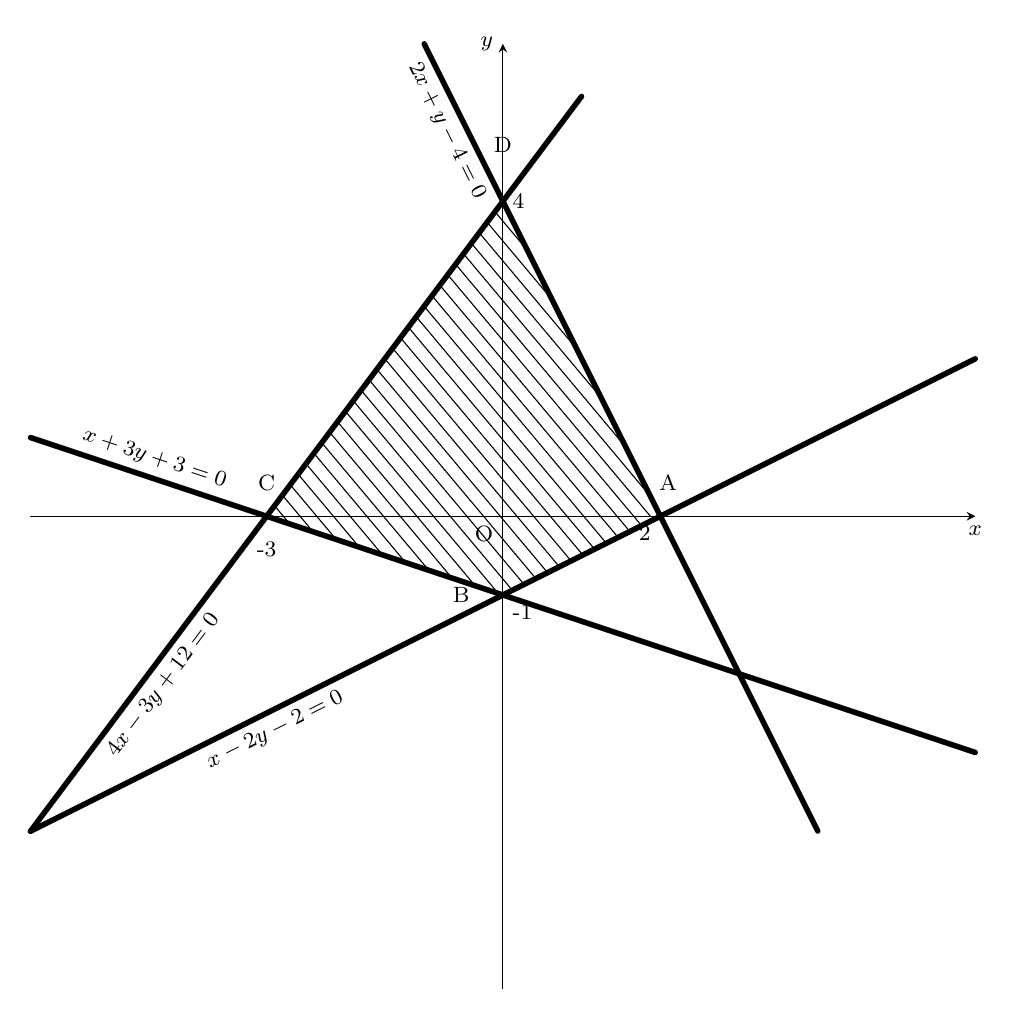
\begin{tikzpicture}[scale=1, font=\footnotesize, line join=round, line cap=round, >=stealth]
				\draw[->] (-6,0)--(6,0) node[below]{$x$};
				\draw[->] (0,-6)--(0,6) node[left]{$y$};
				\begin{scope}%tô màu miền nghiệm
					\clip (-3,0)--(0,-1)--(2,0)--(0,4)--cycle;
					\foreach \x in {-4,-3.9,...,0}{
						\pgfmathsetmacro{\y}{(4*\x/3  +4}
						\draw (\x,\y)--++(-50:4);
					}
				\end{scope}
				\draw[line width=2,black,smooth,samples=100,domain=-6:6] plot(\x,{.5*\x -1});%đường thứ 1
				\path (-6,-4)--(0,-1) node[pos=.5,sloped,below,black]{$x-2y-2=0$}; %tên đường thứ nhất
				\draw[line width=2,black,smooth,samples=100,domain=-6:1] plot(\x,{(4*\x/3  +4});%đường thứ 2
				\path (-6,-4)--(-3,0) node[pos=.5,sloped,below,black]{$4x-3y+12=0$}; %tên đường thứ 2
				\draw[line width=2,black,smooth,samples=100,domain=-6:6] plot(\x,{(-1/3)*\x  -1});%đường thứ 3
				\path (-6,1)--(-3,0) node[pos=.5,sloped,above,black]{$x+3y+3=0$}; %tên đường thứ 3
				\draw[line width=2,black,smooth,samples=100,domain=-1:4] plot(\x,{(-2)*\x  +4});%đường thứ 4
				\path (-1,6)--(0,4) node[pos=.5,sloped,below,black]{$2x+y-4=0$}; %tên đường thứ 4
				\path
				(0,0) node[below left]{O}
				(-3,-0.2) node[below, scale=1]{-3}
				(-3,0.2) node[above, scale=1]{C}
				(0,-1) node[below right,scale=1]{-1}
				(-0.3,-1) node[left,scale=1]{B}
				(2,0) node[below left, scale=1]{2}
				(2.1,0.2) node[above, scale=1]{A}
				(0,4) node[right,scale=1]{4}
				(0,4.5) node[above,scale=1]{D};
			\end{tikzpicture}
		\end{center}
		\begin{itemize}
			\item[•] Tại $A(2;0)$, ta có $F=4\cdot2+5\cdot0-6=2.$
			\item[•] Tại $B(0;-1)$, ta có $F=4\cdot0+5\cdot(-1)-6=-11.$
			\item[•] Tại $C(-3;0)$, ta có $F=4\cdot(-3)+5\cdot0-6=-18.$
			\item[•] Tại $D(0;4)$, ta có $F=4\cdot0+5\cdot4-6=14.$
		\end{itemize}
		Vậy $\max F=14$. }
\end{ex}

\begin{ex}%[0D4T4]
	Một cửa hàng làm kệ sách và bàn làm việc. Mỗi kệ sách cần 5 giờ chế biến gỗ và 4 giờ hoàn thiện. Mỗi bàn làm việc cần 10 giờ chế biến gỗ và 3 giờ hoàn thiện. Mỗi tháng cửa hàng có 600 giờ lao động để chế biến gỗ và 240 giờ để hoàn thiện. Lợi nhuận của mỗi kệ sách là 400 nghìn đồng và mỗi bàn là 750 nghìn đồng. Có bao nhiêu sản phẩm mỗi loại cần được làm mỗi tháng để thu được lợi nhuận tối đa?
	\choice
	{$24000$}
	{$45000$}
	{\True $45600$}
	{$46000$}
	\loigiai{
		\immini{Ta có hệ: $\heva{& 5x+10y\le 600 \\ & 4x+3y\le 240 \\ & x\ge 0 \\ & y\ge 0}$\\
			Lợi nhuận $P=400x+750y$.\\
			Miền nghiệm của hệ là miền tứ giác $OABC$ với
			$$A(0;60),\,B(24;48),\,C(60;0)$$
			Thay tọa độ các đỉnh này vào biểu thức $P$ và so sánh kết quả, ta được
			lợi nhuận tối đa $$P_{\max}=P(B)=45600.$$
		}
		{
			\begin{tikzpicture}[>=stealth', scale=0.05]
				\def\xmin{-10} \def\xmax{140}
				\def\ymin{-10} \def\ymax{100}
				\clip(\xmin,\ymin) rectangle (\xmax,\ymax);
				\tkzDefPoints{\xmax/\ymax/A1,\xmin/\ymax/A2,\xmin/\ymin/A3,\xmax/\ymin/A4}
				\fill[pattern=north east lines,pattern color=blue!60] (A1)--(A2)--(A3)--(A4)--cycle;
				\tkzDefPoints{0/0/O,0/60/A,24/48/B,60/0/C}
				\fill[color=white] (O)--(A)--(B)--(C)--cycle;
				\tkzDrawPoints(A,B,C)
				\draw[domain=-10:140] plot(\x,{60-(\x)/2}) plot(\x,{80-4*(\x)/3});
				\begin{scriptsize}
					\draw[->](\xmin,0)--(\xmax,0); \draw(\xmax-4,0) node[below]{$x$};
					\draw[->](0,\ymin)--(0,\ymax); \draw(0,\ymax-4) node[right]{$y$};
					\draw node [below left]{$O$};
				\end{scriptsize}
			\end{tikzpicture}
		}
	}
\end{ex}

\begin{ex}%[0D4K4-3]
	Khẩu phần dinh dưỡng hàng ngày cho người ăn kiêng cần cung cấp ít nhất $300$ calo, $36$ đơn vị vitamin $A$ và $90$ đơn vị vitamin $C$. Một tách thức uống $X$ có giá $5$ nghìn đồng và cung cấp $60$ calo, $12$ đơn vị vitamin $A$ và $10$ đơn vị vitamin $C$. Một tách thức uống $Y$ có giá $6$ nghìn đồng và cung cấp $60$ calo, $6$ đơn vị vitamin $A$ và $30$ đơn vị vitamin $C$. Mỗi ngày nên uống bao nhiêu tách mỗi loại để có được chi phí tối ưu và vẫn đáp ứng được yêu cầu dinh dưỡng hàng ngày?
	\choice
	{$1$ tách loại $X$, $4$ tách loại $Y$}
	{\True $3$ tách loại $X$, $2$ tách loại $Y$}
	{$2$ tách loại $X$, $3$ tách loại $Y$}
	{$4$ tách loại $X$, $1$ tách loại $Y$}
	\loigiai{
		\immini{
			Ta có hệ: $\heva{& 60x+60y\ge 300 \\ & 12x+6y\ge 36 \\ & 10x+30y \ge 90 \\& x\ge 0 \\ & y\ge 0}$\\
			Giá $C=5x+6y$.\\
			Miền nghiệm như hình vẽ. Các đỉnh là:\\
			$M(0;6)$, $N(1;4)$, $P(3;2)$, $Q(9;0)$.\\
			$C$ nhỏ nhất tại đỉnh $P(3;2)$.\\
			Vậy nên uống $3$ tách loại $X$ và $2$ tách loại $Y$.
		}
		{
			\begin{tikzpicture}[scale=0.5, font=\footnotesize, line join=round, line cap=round, >=stealth]
				\def\xmin{-2} \def\xmax{12}
				\def\ymin{-2} \def\ymax{8}
				\clip(\xmin,\ymin) rectangle (\xmax,\ymax);
				\tkzDefPoints{\xmax/\ymax/A1,\xmin/\ymax/A2,\xmin/\ymin/A3,\xmax/\ymin/A4}
				\tkzDefPoints{0/6/M,1/4/N,3/2/P,9/0/Q}
				\tkzDrawPoints(M,N,P,Q) \tkzLabelPoints[above right](M,N,P,Q)
				
				\fill[pattern=north east lines,pattern color=black!60] (A2)--(A3)--(A4)--(\xmax,0)--(Q)--(P)--(N)--(M)--(0,\ymax)--cycle;
				\draw[domain=-2:12] plot(\x,{5-(\x)}) plot(\x,{6-2*(\x)}) plot(\x,{3-(\x)/3});
				\begin{scriptsize}
					\draw[->](\xmin,0)--(\xmax,0); \draw(\xmax-0.1,0) node[below]{$x$};
					\draw[->](0,\ymin)--(0,\ymax); \draw(0,\ymax-0.2) node[right]{$y$};
					\foreach \x in {2,4,6,8,10}
					\draw (\x,0.05) -- ++(0,-0.1) node [below] {$\x$};
					\foreach \x in {2,4,6,8}
					\draw (0.05,\x) -- ++(-0.1,0) node [left] {$\x$};
					\draw node [below left]{$O$};
				\end{scriptsize}
			\end{tikzpicture}
		}	
	}
\end{ex}

\begin{ex}%[0D4T4]
	Người ta dự định dùng hai loại nguyên liệu để chiết xuất ít nhất $140$ kg chất A và $9$ kg chất B. Từ mỗi tấn nguyên liệu loại I giá $4$ triệu đồng, có thể chiết xuất được $20$ kg chất A và $0,6$ kg chất B. Từ mỗi tấn nguyên liệu loại II giá $3$ triệu đồng có thể chiết xuất được $10$ kg chất A và $1,5$ kg chất B. Hỏi phải dùng bao nhiêu tấn nguyên liệu mỗi loại để chi phí mua nguyên liệu là ít nhất, biết rằng cơ sở cung cấp nguyên liệu chỉ có thể cung cấp không quá $10$ tấn nguyên liệu loại I và không quá $9$ tấn nguyên liệu loại II?
	\choice
	{$2,5$ tấn loại I và $9$ tấn loại II}
	{$10$ tấn loại I và $9$ tấn loại II}
	{$10$ tấn loại I và $2$ tấn loại II}
	{\True $5$ tấn loại I và $4$ tấn loại II}
	\loigiai{
		Gọi $x$, $y$ lần lượt là số tấn nguyên liệu loại I và loại II phải dùng.\\
		Từ bài toán ta đưa được hệ bất phương trình:
		$\heva{&0 \leq x \leq 10\\&0 \leq y \leq 9\\&2x+y\geq 14\\&2x+5y\geq 30} (*)$\\
		Tổng chi phí là $F(x;y)=4x+3y$\\
		Ta tìm $x$, $y$ thỏa mãn hệ $(*)$ sao cho $F(x;y)$ nhỏ nhất.
		\begin{center}
			\begin{tikzpicture}[scale=0.7,thick,>=stealth']
				\draw[->] (-1,0) -- (15.3,0)node[above]{$x$};
				\foreach \x in {1,2,3,4,5,6,7,8,9,10,11,12,13,14,15}
				\draw[shift={(\x,0)},color=black] (0pt,2pt) -- (0pt,-2pt) node[below] {\footnotesize $\x$};
				\draw[->,color=black] (0,-1) -- (0,14.3)node[right]{$y$};
				\foreach \y in {1,2,3,4,5,6,7,8,9,10,11,12,13,14}
				\draw[shift={(0,\y)},color=black] (2pt,0pt) -- (-2pt,0pt) node[left] {\footnotesize $\y$};
				\node[below left] at (0,0) {$O$};
				\clip(-1,-1) rectangle (15.3,14.3);
				\fill[pattern=north east lines] (-0.15,14.3) -- (-1,14.3) -- (-1,-1) -- (7.5,-1)-- cycle;
				\draw[line width=1.2pt,smooth,samples=100,domain=-1:9] plot(\x,{14-2*(\x)});
				\fill[pattern=north east lines] (-1,6.4)--(-1,-1)--(15.3,-1)--(15.3,-0.12)-- cycle;
				\draw[line width=1.2pt,smooth,samples=100,domain=-1:15.3] plot(\x,{6-0.4*(\x)});
				\fill[pattern=north east lines] (-1,9)--(-1,14.3) --(15.3,14.3)--(15.3,9)-- cycle;
				\draw[line width=1.2pt,smooth,samples=100,domain=-1:15.3] plot(\x,{9+0*(\x)});
				\fill[pattern=north east lines] (10,14.3)--(15.3,14.3) --(15.3,-1)--(10,-1)-- cycle;
				\draw[line width=1.2pt,smooth,samples=100](10,-1)--(10,15.3);
				\fill[pattern=north east lines] (0,4)--(-3,4) --(-3,-3)--(0,-3)-- cycle;
				\draw[line width=1.2pt,smooth,samples=100,domain=-3:9] plot(\x,{0*(\x)});
				\node[left] at (5.5,4.5) {$A$};
				\node[left] at (10,3) {$B$};
				\node[left] at (10,9) {$C$};
				\node[right] at (2.75,9) {$D$};	
			\end{tikzpicture}
		\end{center}
		Ta biết giá trị nhỏ nhất đạt tại các điểm $A(5;4)$, $B(10;2)$, $C(10;9)$, $D(3;9)$.\\
		Thử lại thấy $F(5;4)$=32 là giá trị nhỏ nhất.\\
		Vậy cần 5 tấn nguyên liệu loại I và 4 tấn nguyên liệu loại II.
	}
\end{ex}

\begin{ex}%[0D4K4-3]
	Một nhà máy sản xuất, sử dụng ba loại máy đặc chủng để sản xuất sản phẩm $A$ và sản phẩm $B$ trong một chu trình sản xuất. Đề sản xuất một tấn sản phẩm $A$ lãi $4$ triệu đồng người ta sử dụng máy $I$ trong 1 giờ, máy II trong $2$ giờ và máy III trong $3$ giờ. Để sản xuất ra một tấn sản phẩm $B$ lãi được $3$ triệu đồng người ta sử dụng máy I trong $6$ giờ, máy II trong $3$ giờ và máy III trong $2$ giờ. Biết rằng máy $I$ chỉ hoạt động không quá $36$ giờ, máy hai hoạt động không quá $23$ giờ và máy III hoạt động không quá $27$ giờ. Hãy lập kế hoạch sản xuất cho nhà máy để tiền lãi được nhiều nhất. 
	\choice
	{Sản xuất $9$ tấn sản phẩm $A$ và không sản xuất sản phẩm $B$}
	{Sản xuất $7$ tấn sản phẩm $A$ và $3$ tấn sản phẩm $B$}
	{\True Sản xuất $\dfrac{45}{8}$ tấn sản phẩm $A$ và $\dfrac{81}{16}$ tấn sản phẩm $B$}
	{Sản xuất $6$ tấn sản phẩm $B$ và không sản xuất sản phẩm $A$}
	\loigiai{
		Gọi $x \geq 0$, $y \geq 0$ (tấn) là sản lượng cần sản xuất của sản phẩm $A$ và sản phẩm $B$. Ta có:\\
		$x+6 y$ là thời gian hoạt động của máy I,\\
		$2 x+3 y$ là thời gian hoạt động của máy II,\\
		$3 x+2 y$ là thời gian hoạt động của máy III.
		Số tiền lãi của nhà máy: $T=4 x+3 y$ (triệu đồng).
		Bài toán trở thành: Tìm $x \geq 0$, $y \geq 0$ thỏa mãn $\heva{&x+6 y \leq 36 \\ &2 x+3 y \leq 23 \\ &3 x+2 y \leq 27}$ để $T=4 x+3 y $ đạt giá trị lớn nhất.\\
		Miền nghiệm của hệ trên là tam giác $ABC$ (kể cả bờ).
		\begin{center}
			\begin{tikzpicture}[line cap=round,line join=round,>=stealth,x=1.0cm,y=1.0cm,scale=.7]
				\clip(-1,-1.5) rectangle (10,7);
				\draw[->] (-1,0) -- (10,0) node[above left]{$x$};
				\draw[->] (0,-1.5) -- (0,7)node[below right]{$y$};
				\draw[smooth,samples=100,domain=-1:10] plot(\x,{(--36-1*\x)/6});
				\draw[smooth,samples=100,domain=-1:10] plot(\x,{(--23-2*\x)/3});
				\draw[smooth,samples=100,domain=-1:10] plot(\x,{(--27-3*\x)/2});
				\fill[pattern=north east lines] (-1,-1.5) -- (-1,7) -- (10,7) -- (10,-1.5) -- cycle;
				\draw [fill=white] (3.33,5.44) -- (5.63,5.06) -- (7,3) -- cycle;
				\fill (0,0)node[above left]{$O$}circle(1.2pt) (3.33,5.44)node[above]{$A$}circle(1.2pt) (5.63,5.06)node[above right]{$B$}circle(1.2pt) (7,3)node[above right]{$C$}circle(1.2pt);
				\draw[fill=black] (5.63,0) node[below]{$\dfrac{45}{8}$} (0,5.06)node[left]{$\dfrac{81}{16}$};
				\draw[dashed] (5.63,0) |- (5.63,5.06) |- (0,5.06);
			\end{tikzpicture}
		\end{center}
		Xét tại các vị trí $A\left(\dfrac{10}{3};\dfrac{49}{9}\right)$, $B\left(\dfrac{45}{8};\dfrac{81}{16}\right)$, $C(7;3)$ ta có $f\left(\dfrac{10}{3};\dfrac{49}{9}\right)=\dfrac{89}{3}$, $f\left(\dfrac{45}{8};\dfrac{81}{16}\right)=\dfrac{603}{16}$, $f(7;3)=37$.\\
		Suy ra $f(x;y)$ lớn nhất khi $(x;y)=\left(\dfrac{45}{8};\dfrac{81}{16}\right)$. \\
		Như vậy để tiền lãi được nhiều nhất thì sản xuất $\dfrac{45}{8}$ tấn sản phẩm $A$ và $\dfrac{81}{16}$ tấn sản phẩm $B$.}
\end{ex}

\centerline{\textbf{---HẾT---}}
\Closesolutionfile{ans}